% Version 1.2 of SN LaTeX, November 2022
%
% See section 11 of the User Manual for version history 
%
%%%%%%%%%%%%%%%%%%%%%%%%%%%%%%%%%%%%%%%%%%%%%%%%%%%%%%%%%%%%%%%%%%%%%%
%%                                                                 %%
%% Please do not use \input{...} to include other tex files.       %%
%% Submit your LaTeX manuscript as one .tex document.              %%
%%                                                                 %%
%% All additional figures and files should be attached             %%
%% separately and not embedded in the \TeX\ document itself.       %%
%%                                                                 %%
%%%%%%%%%%%%%%%%%%%%%%%%%%%%%%%%%%%%%%%%%%%%%%%%%%%%%%%%%%%%%%%%%%%%%

%%\documentclass[referee,sn-basic]{sn-jnl}% referee option is meant for double line spacing

%%=======================================================%%
%% to print line numbers in the margin use lineno option %%
%%=======================================================%%

%%\documentclass[lineno,sn-basic]{sn-jnl}% Basic Springer Nature Reference Style/Chemistry Reference Style

%%======================================================%%
%% to compile with pdflatex/xelatex use pdflatex option %%
%%======================================================%%

%%\documentclass[pdflatex,sn-basic]{sn-jnl}% Basic Springer Nature Reference Style/Chemistry Reference Style


%%Note: the following reference styles support Namedate and Numbered referencing. By default the style follows the most common style. To switch between the options you can add or remove “Numbered” in the optional parenthesis. 
%%The option is available for: sn-basic.bst, sn-vancouver.bst, sn-chicago.bst, sn-mathphys.bst. %  
 
%%\documentclass[sn-nature]{sn-jnl}% Style for submissions to Nature Portfolio journals
%%\documentclass[sn-basic]{sn-jnl}% Basic Springer Nature Reference Style/Chemistry Reference Style
\documentclass[sn-mathphys,Numbered]{sn-jnl}% Math and Physical Sciences Reference Style
%%\documentclass[sn-aps]{sn-jnl}% American Physical Society (APS) Reference Style
%%\documentclass[sn-vancouver,Numbered]{sn-jnl}% Vancouver Reference Style
%%\documentclass[sn-apa]{sn-jnl}% APA Reference Style 
%%\documentclass[sn-chicago]{sn-jnl}% Chicago-based Humanities Reference Style
%%\documentclass[default]{sn-jnl}% Default
%%\documentclass[default,iicol]{sn-jnl}% Default with double column layout

%%%% Standard Packages
%%<additional latex packages if required can be included here>

\usepackage{graphicx}%
\usepackage{multirow}%
\usepackage{amsmath,amssymb,amsfonts}%
\usepackage{amsthm}%
\usepackage{mathrsfs}%
\usepackage[title]{appendix}%
\usepackage{xcolor}%
\usepackage{textcomp}%
\usepackage{manyfoot}%
\usepackage{booktabs}%
\usepackage{algorithm}%
\usepackage{algorithmicx}%
\usepackage{algpseudocode}%
\usepackage{listings}%
%%%%

%%%%%=============================================================================%%%%
%%%%  Remarks: This template is provided to aid authors with the preparation
%%%%  of original research articles intended for submission to journals published 
%%%%  by Springer Nature. The guidance has been prepared in partnership with 
%%%%  production teams to conform to Springer Nature technical requirements. 
%%%%  Editorial and presentation requirements differ among journal portfolios and 
%%%%  research disciplines. You may find sections in this template are irrelevant 
%%%%  to your work and are empowered to omit any such section if allowed by the 
%%%%  journal you intend to submit to. The submission guidelines and policies 
%%%%  of the journal take precedence. A detailed User Manual is available in the 
%%%%  template package for technical guidance.
%%%%%=============================================================================%%%%

%\jyear{2021}%
\raggedbottom
%%\unnumbered% uncomment this for unnumbered level heads

\begin{document}

\title[Article Title]{Supplementary Material for ``Developing Comprehensive Annotation Guidelines and a Corpus of Risk of Bias Assessment for Rehabilitation: A Methodological Approach''}

%%\pacs[JEL Classification]{D8, H51}

%%\pacs[MSC Classification]{35A01, 65L10, 65L12, 65L20, 65L70}

\maketitle


%%%%%%%%%%%%%%%%
%% Background %%
\section*{Generic annotation guidelines}
\label{sec:generic}
%
In each of the following subsections, we describe the annotation guidelines for the signalling questions using the instructional placards developed through consultation with RoB assessment and natural language processing experts.

Each placard is a flowchart encoding instructions to guide annotators in annotating the RoB question by question for the signalling questions in the Revised Cochrane RoB tool 2.0.
The flowchart starts with the title informing the annotators of which question they are annotating for.
The first diamond in the actual instructional flowchart asks the annotators to look for specific information or part of the text and, if found, instructs them to annotate it.
There are little colour-coded arrows flanking the diamond instructing the annotators to first look for the information in the green arrow region (for e.g., in the Results section). 
If the information is not found in the green-coded arrow, check for it in the yellow-coded arrow (e.g., a table or a flowchart).
If for a particular question, no information is found, we assume that the text did not have any information for that particular signalling question.
\textcolor{red}{Include a generic description about the colours, logos, shapes and flowchart elements in the placards here...}
%
%
%
\section*{Annotation Guidelines for RoB domain 1}
\label{sec:dom1}
%
The first risk domain of bias in the revised Cochrane Risk of Bias (RoB) 2.0 tool is "Bias arising from the randomization process" which includes the subdomains "Random sequence generation" and "Allocation concealment". This domain assesses the potential for bias related to the randomization process, which is an important factor in reducing the risk of selection bias in randomized controlled trials (RCTs).
%
%
%
\subsection*{Signalling question: 1.1}
%
Follow the Flowchart~\ref{fig:1_1} for annotation instructions of the signalling question, ``Was the allocation sequence random?''.
%
\begin{figure}[hbt]
    \centering
    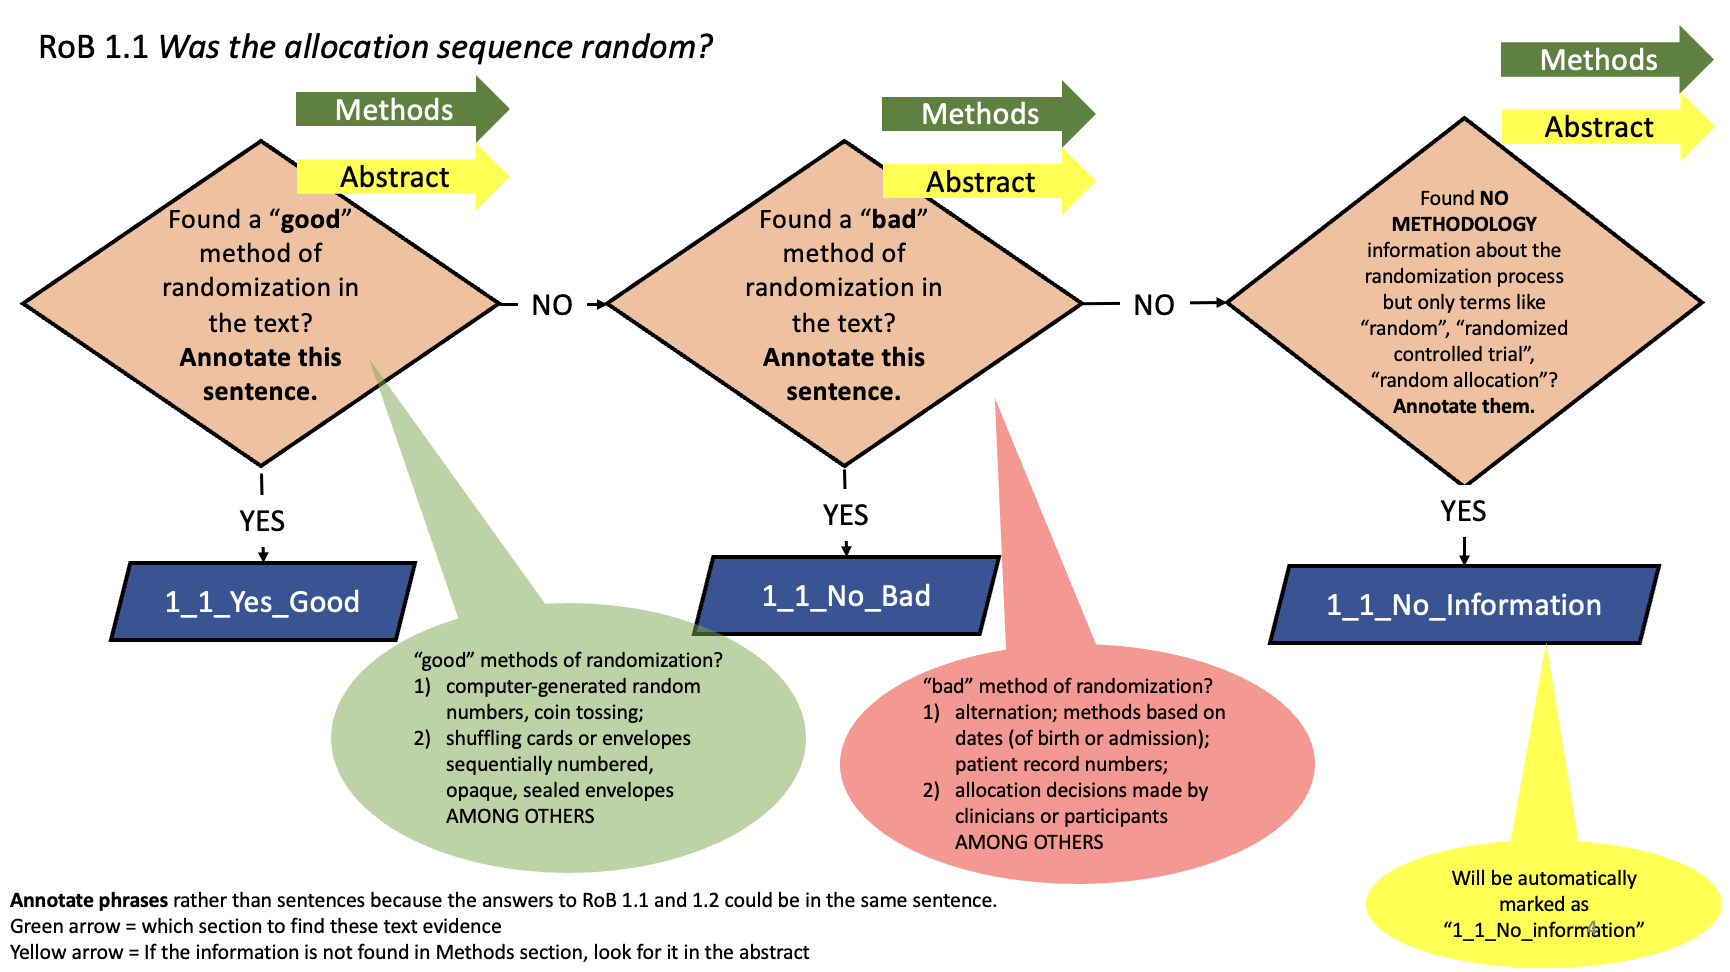
\includegraphics[width=\textwidth]{figures/1_1.png}
    \caption{Annotation instructions for the RoB 1.1 signalling question.}
    \label{fig:1_1}
\end{figure}

%
If the allocation sequence is generated randomly, this reduces the risk of bias, as it ensures that the allocation is not influenced by the researchers' preferences or the participants' characteristics.
Some of the good random allocation methods include Simple randomization (coin flipping, random number generator), stratified randomization, blocked randomization, cluster randomization, and adaptive randomization.
If the allocation sequence was not generated using a proper randomization method, this increases the risk of bias in the study.
For e.g., if the allocation sequence was generated using a non-random method, such as alternating assignment or assignment based on participant characteristics, this could introduce bias into the study.
Following this explanation, the first diamond in the flowchart~\ref{fig:1_1}, instructs the annotators to identify randomization method for allocation sequence and if a proper randomization method is found, mark the method (this should be a few words or a phrase and not a complete sentence) with ``1.1 Yes Good''.
If the text describes a bad or improper method of randomization, mark the text with ``1.1 No Bad''.
If you did not find any information about the randomization methodology, but found terms like ``random'', ``randomized trial'' or phrases like ``we did random allocation'', then mark such phrases with label ``1.1 No Information''.
The information about random sequence allocation could be found in the methods section (first priority) or the abstract (second priority).
Notice that for this signalling question, the annotators are required to mark phrases rather than full sentences.
%
%
%
\subsection*{Signalling question: 1.2}
%
Follow the Flowchart~\ref{fig:1_2} for annotation instructions of the signalling question, ``Was the allocation sequence concealed until participants were enrolled and assigned to interventions?''.
%
\begin{figure}[hbt]
    \centering
    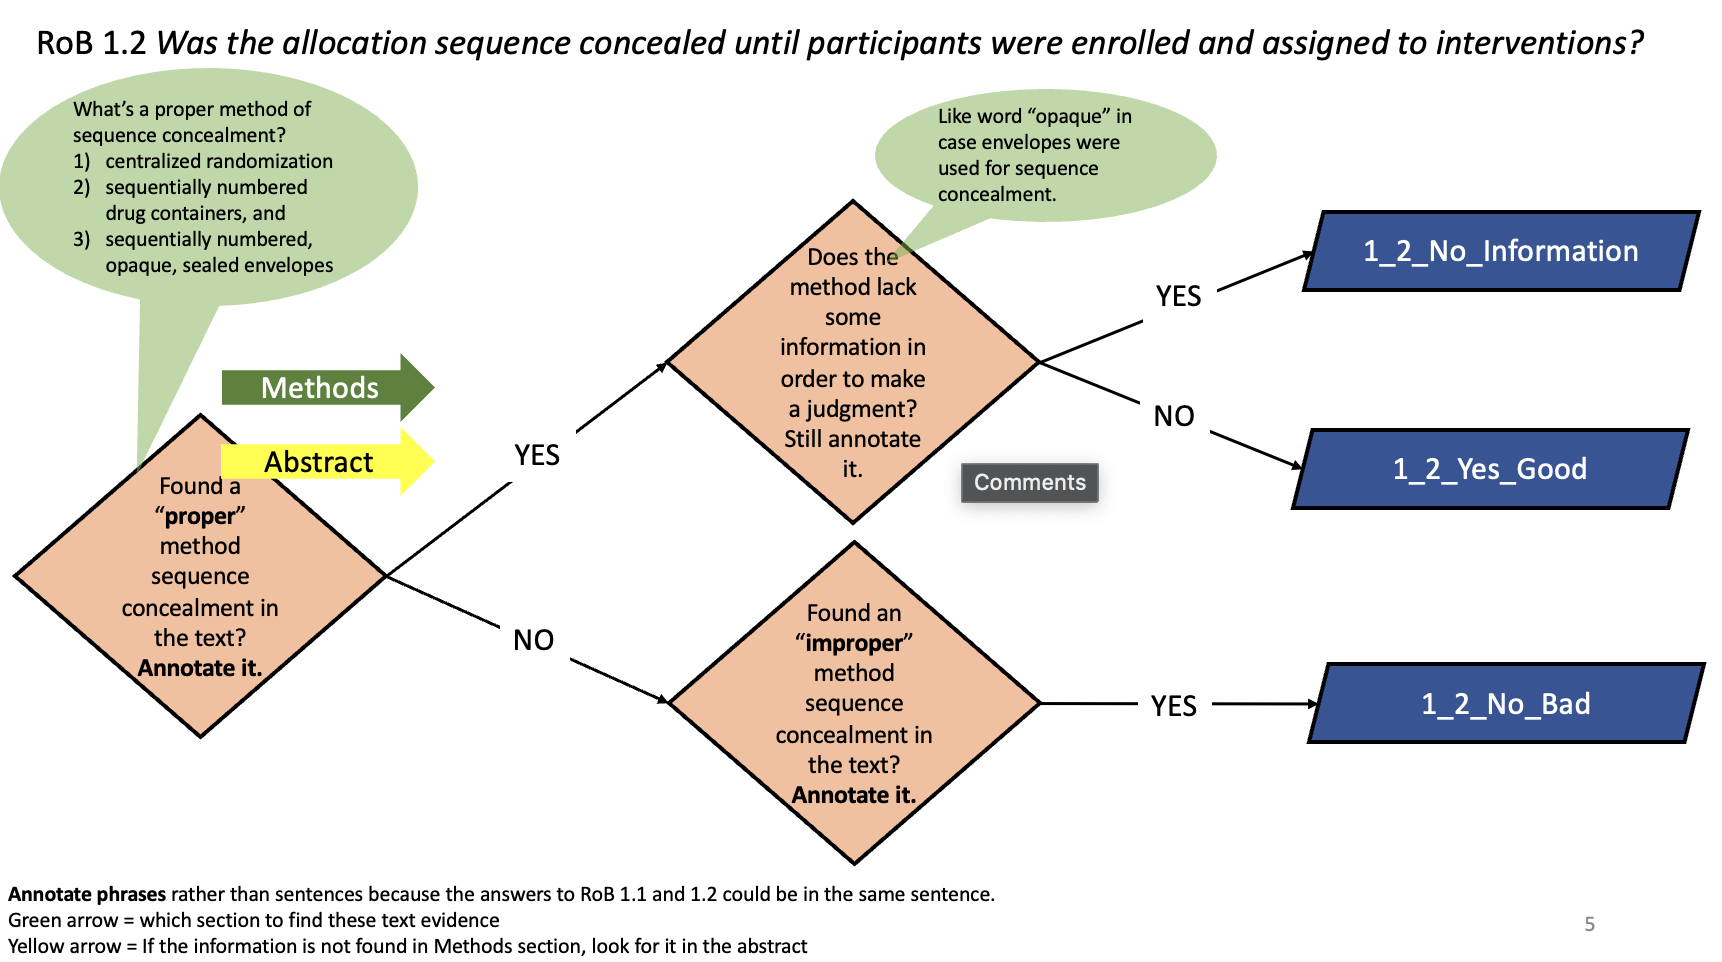
\includegraphics[width=\textwidth]{figures/1_2.png}
    \caption{Annotation instructions for the RoB 1.2 signalling question.}
    \label{fig:1_2}
\end{figure}


In randomized controlled trials (RCTs), the allocation sequence determines the order in which participants are assigned to each intervention group.
Adequate concealment of the allocation sequence refers to the process of keeping the sequence hidden from those who are involved in enrolling and assigning participants to intervention groups.
This helps to prevent the possibility of selection bias, which can occur if those enrolling participants in the trial have knowledge of the allocation sequence and can manipulate the assignment of participants to intervention groups based on that knowledge.
If the allocation sequence is not adequately concealed until participants are enrolled and assigned to interventions, this can increase the risk of bias and may lead to systematic differences between the intervention groups.
For example, if the allocation sequence is known to the investigators or coordinators, they may selectively enroll participants who are more likely to benefit from a particular intervention, or they may assign participants to one intervention group over another based on personal biases or preferences.


The good methods of randomization:
Centralized randomization: This involves using a central unit or an independent third-party to generate and conceal the allocation sequence. This helps to ensure that the allocation sequence is kept hidden from those enrolling and assigning participants to intervention groups.
Sealed opaque envelopes: This involves preparing sealed envelopes with the allocation sequence inside. The envelopes are then kept in a secure location and opened sequentially as participants are enrolled in the trial.
Online randomization tools: This involves using secure online systems to generate and conceal the allocation sequence. The system ensures that the allocation sequence is not visible to those enrolling and assigning participants to intervention groups.

The bad methods of randomization:
Using an open list: This involves using a visible list of randomization codes, which allows those enrolling and assigning participants to intervention groups to see the allocation sequence. This method does not provide adequate concealment of the allocation sequence and increases the risk of selection bias.

Using a predictable sequence: This involves using a predictable sequence to allocate participants to intervention groups, such as alternating between groups or using birth dates to determine group assignment. This method does not provide adequate concealment of the allocation sequence and increases the risk of selection bias.

Using the participant's choice: This involves allowing participants to choose their intervention group. This method does not provide adequate concealment of the allocation sequence and increases the risk of selection bias, as participants may choose the intervention group based on personal preferences or expectations.


Following this explanation, the first diamond in the flowchart~\ref{fig:1_2}, instructs the annotators to identify method of allocation concealment and if a proper concealment method is found, mark the method (this should be a few words or a phrase and not a complete sentence) with ``1.2 Yes Good''.
If you found text describing the method of allocation concealment but it lacks some information to make judgment, then label the marked text as ``1.2 No Information''.
If the text describes a bad or improper method of allocation concealment, mark the text with ``1.2 No Bad''.
The information about allocation concealment could be found in the methods section (first priority) or the abstract (second priority).
Notice that for this signalling question too, the annotators are required to mark phrases rather than full sentences.
%
%
%
\subsection*{Signalling question: 1.3}
%
Follow the Flowchart~\ref{fig:1_3} for annotation instructions of the signalling question, ``Did baseline differences between intervention groups suggest a problem with the randomization process?''.
%

\begin{figure}[hbt]
    \centering
    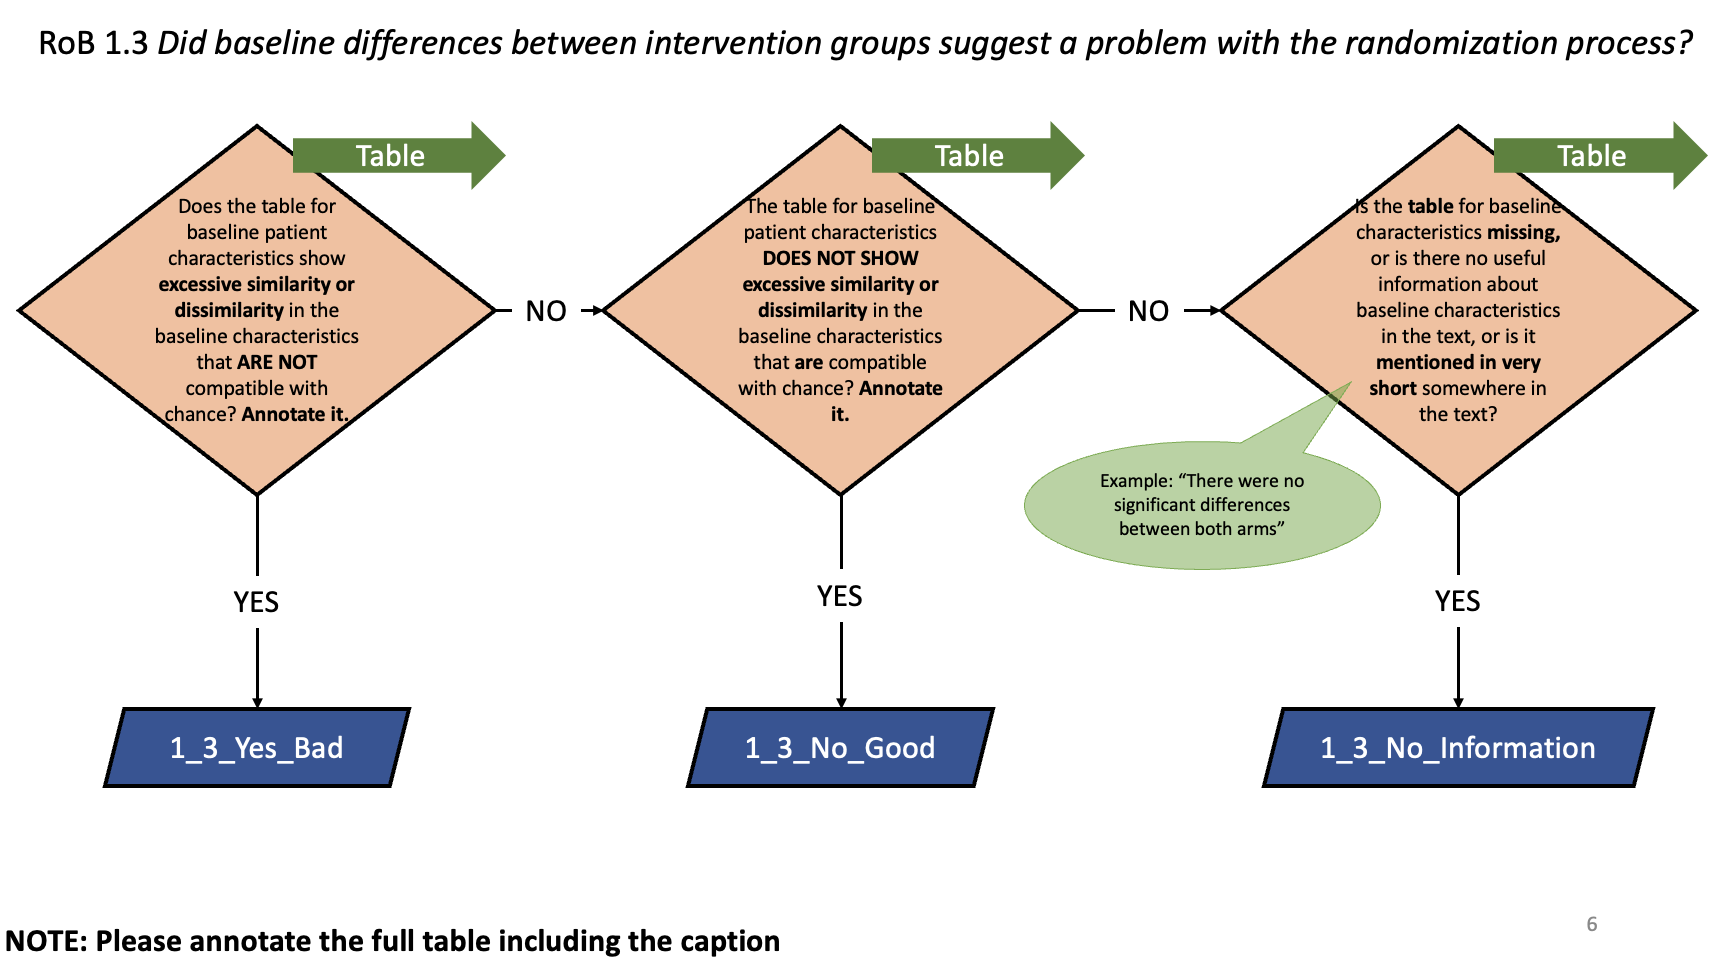
\includegraphics[width=\textwidth]{figures/1_3.png}
    \caption{Annotation instructions for the RoB 1.3 signalling question.}
    \label{fig:1_3}
\end{figure}

%

The bias assessed by the "Bias arising from baseline measurements" domain and subdomain ``Did baseline differences between intervention groups suggest a problem with the randomization process?'' of the revised Cochrane Risk of Bias (RoB) 2.0 tool is related to the potential for bias arising from differences in baseline characteristics between intervention groups that are not related to chance and may suggest a problem with the randomization process.
Randomization is a critical aspect of RCTs because it helps to ensure that the intervention groups are comparable at baseline, meaning that any differences observed between groups after the intervention can be attributed to the intervention itself rather than other factors.
However, even with randomization, chance imbalances in baseline characteristics can occur.
The question addressed by this subdomain is whether any differences in baseline characteristics between intervention groups suggest that the randomization process was not effective.
For example, if the intervention group has significantly more female participants, older participants, or participants with more severe disease at baseline compared to the control group, this may suggest that the randomization process was not effective or that there was a problem with the allocation sequence.
This can lead to biased estimates of treatment effects and decrease the internal validity of the study.
Therefore, the Cochrane RoB 2.0 tool assesses the potential for bias arising from baseline differences between intervention groups to help determine the risk of bias related to the randomization process.
If there are significant differences in baseline characteristics between intervention groups that are not related to chance, this may suggest that the randomization process was not effective, and the reliability of the study results may be decreased.


The text describing answer to this question is typically found in the table describing demographic and clinical baseline characteristics of study participants.
If the table for baseline patient characteristics show excessive similarity or dissimilarity in the baseline characteristics that ARE NOT compatible with chance then mark the full table with label ``1.3 Yes Bad'' other mark the full table and the table caption with label ``1.3 No Good''.
If you did not find any table describing the baseline patient characteristics then the study will be ultimately assumed as ``1.3 No Information''.
At this point, we request the annotators to mark the full table instead of one or two characteristics.
This is because we will only use text extracted from PDFs to train the machine learning model that could predict on text and the not the PDF (like RobotReviewer).
Apart from the table, there could be text description that could hint towards baseline differences that could act as confounding factors.
For instance, consider the following sentence, ``Because baseline ODI differences were a potential confounding factor, an adjusted multiple linear and logistic regression analysis was performed for each continuous and categorical outcome measure, respectively.'' (Cohen, Steven P., et al. "Randomized placebo-controlled study evaluating lateral branch radiofrequency denervation for sacroiliac joint pain." The Journal of the American Society of Anesthesiologists 109.2 (2008): 279-288.)


%
%
%
\section*{Annotation Guidelines for RoB domain 2}
\label{sec:dom2}
%
Before detailing annotation instructions for this domain, we clarify the difference between deviations from intended interventions and dropouts from the trial.
Deviations from intended interventions are any unintentional changes that could have occurred in the intervention under investigation in the trial.
For example, participants may not have complied with the study protocol, or there might have been problems with the delivery of the intervention that could have influenced the study outcomes.
In contrast, dropouts refer to participants who withdrew from the study or were lost to follow-up.
Dropouts can potentially introduce bias into a study if the characteristics of the participants who dropped out are different from those who completed the study.
High dropout rates can also affect the statistical power of the study and its ability to draw valid conclusions.
Although both deviations from the intended intervention and dropout rates can potentially introduce bias into a study, they are not the same thing and should be evaluated separately when assessing the risk of bias in a study.
%
%
%
\subsection*{Signalling question - 2.1}
\label{subsec:2_1}
%

%

\begin{figure}[hbt]
    \centering
    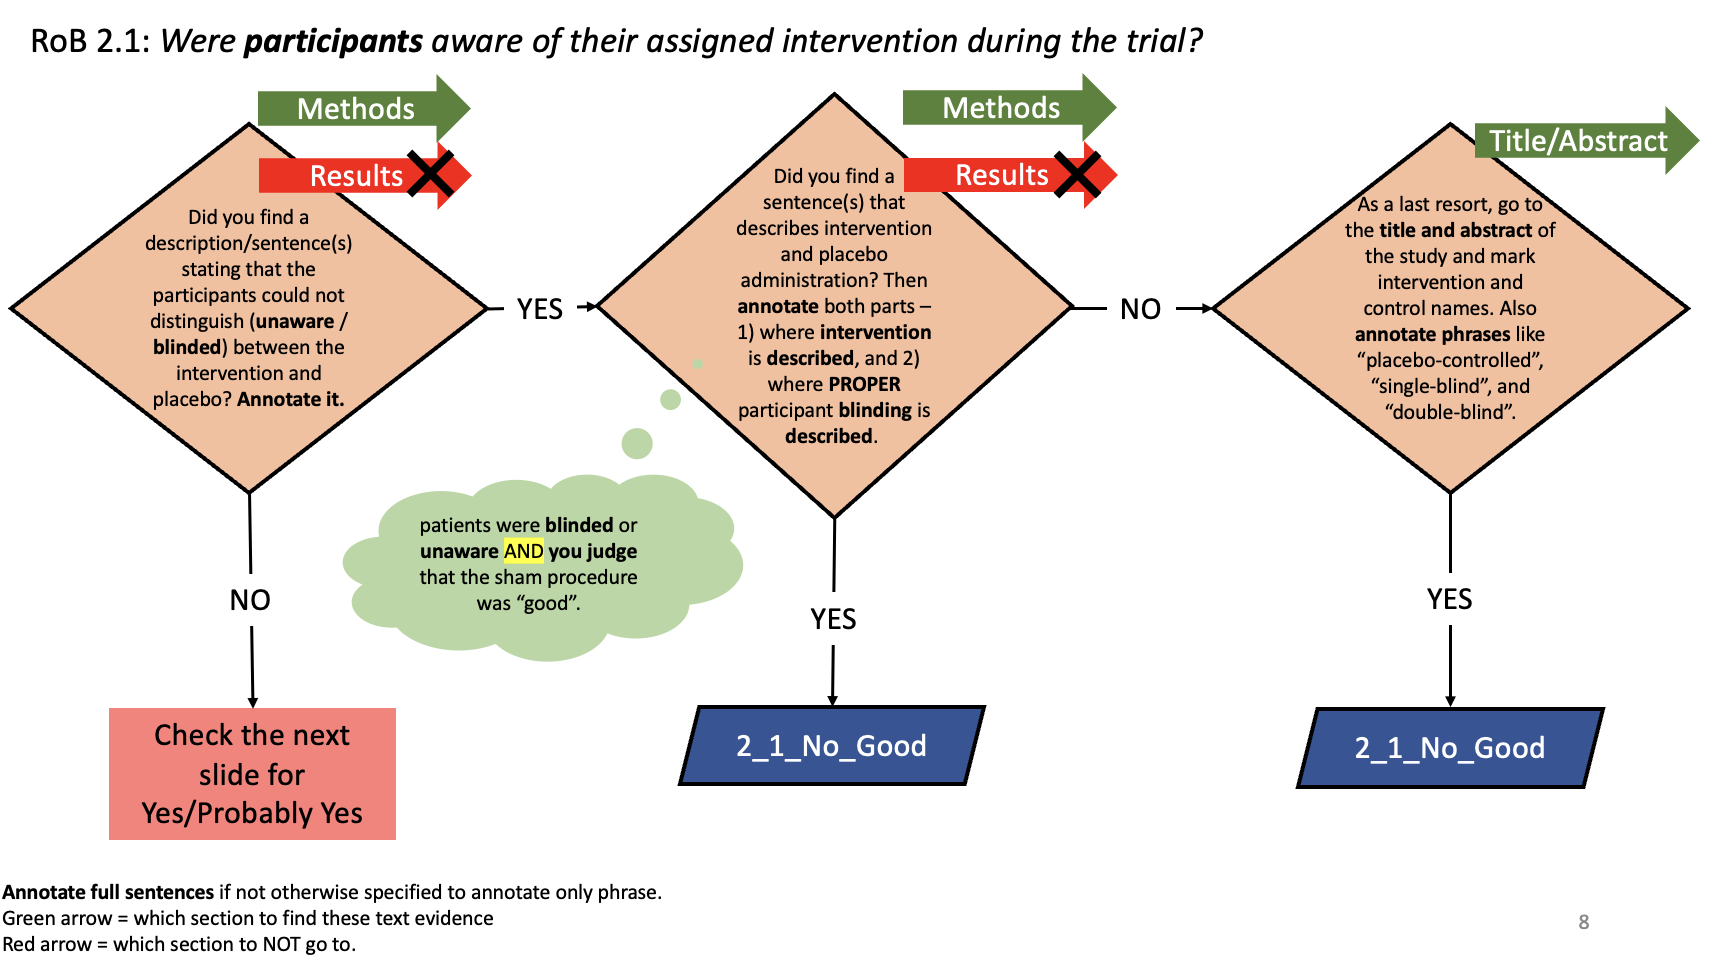
\includegraphics[width=\textwidth]{figures/2_1.png}
    \caption{Annotation instructions for the RoB 2.1 signalling question.}
    \label{fig:2_1}
\end{figure}
\begin{figure}[hbt]
    \centering
    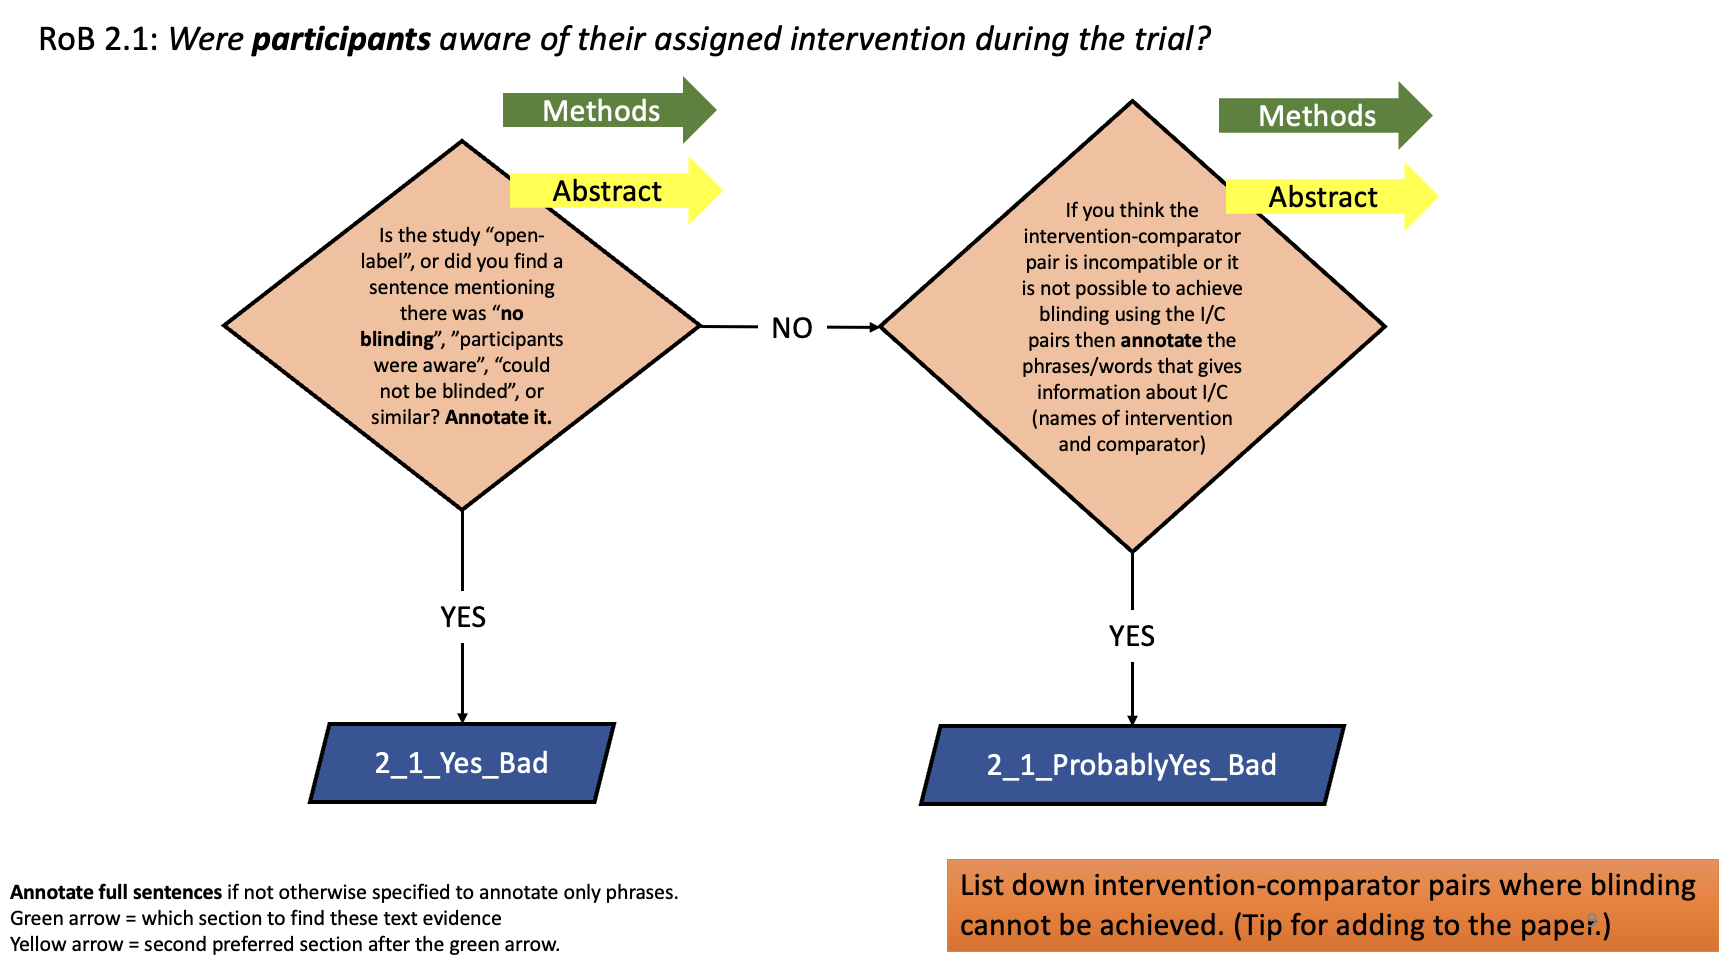
\includegraphics[width=\textwidth]{figures/2_1_1.png}
    \caption{Annotation instructions for the RoB 2.1 signalling question.}
    \label{fig:2_1_1}
\end{figure}
%
Blinding or masking of participants is an essential method to minimize the risk of bias due to participants' knowledge of their assigned intervention.
When participants are not blinded, they may modify their behavior, expectations, or reports of outcomes, consciously or unconsciously, based on their knowledge of the assigned intervention, leading to a biased estimate of treatment effect.
If blinding was applied to the participants, the risk of bias related to the knowledge of the assigned intervention is minimized.
If participants were not blinded and were aware of their assigned intervention, this may increase the risk of bias and decrease the reliability of the study results.
However, if blinding was successfully applied, this may decrease the risk of bias and increase the internal validity of the study.


Following this explanation, the annotators are asked to find text description/sentence(s) stating that the participants could not distinguish (unaware / blinded) between the intervention and placebo.
If the annotators found sentence(s) that describe intervention and placebo administration, then they are asked to annotate both parts – first part where intervention is described, and second part where proper participant blinding is described.
Annotate these parts with the label ``2.1 No Good''.
Proper blinding of participants involves concealing or disguising the intervention to ensure that the participants do not know which intervention they received.
These are the proper methods of blinding.
Use of placebo or sham interventions: In some rehabilitation trials, a placebo or sham intervention can be used to blind the participants and therapists to the assigned intervention. For example, in studies of manual therapy, a sham therapy such as light touch or a placebo intervention like ultrasound can be used to blind the participants.

Use of standardized interventions: Standardized interventions can be used to ensure that all participants receive the same intervention regardless of the assigned group. This approach helps reduce the risk of bias and ensures that all participants receive the same level of care.

Use of therapist blinding: In some rehabilitation trials, therapists can be blinded to the assigned intervention. This approach is particularly useful when the intervention involves physical contact with the participant. For example, in studies of physical therapy, therapists can be trained to provide the same level of care and attention to all participants, regardless of the assigned intervention.

Use of remote monitoring: In some rehabilitation trials, interventions can be delivered remotely, using telehealth or other technology. This approach can help blind the participants and therapists to the assigned intervention.

Use of masking techniques: In some rehabilitation trials, masking techniques can be used to conceal the intervention from the participants and therapists. For example, in studies of balance training, participants can be blindfolded to prevent them from seeing the type of training they are receiving.

In summary, blinding in rehabilitation trials can be challenging, but several methods can be used to minimize the risk of bias due to the knowledge of the assigned intervention by the study participants and therapists. These methods include the use of placebo or sham interventions, standardized interventions, therapist blinding, remote monitoring, and masking techniques.



Annotators are likely to find this information in the methods section.
If the information is not found in the Methods section, but there are phrases in title saying ``placebo-controlled'', ``single-blind'', ``double-blind'', then mark these phrases with label ``2.1 No Good''.

If you did not find any such information then did you find texts saying that the study is ``open-label'', or did you find a sentence mentioning there was no blinding, or participants were aware, or could not be blinded, or something along the lines of the sentences mentioned below, then annotate such sentences with the label ``2.1 Yes Bad''.
1. Due to the nature of the intervention, it was not possible to blind the participants to their assigned group.
2. The physical nature of the intervention made it impossible to blind the participants to their assigned group.
3. Participants were not blinded to their assigned group as the intervention required direct physical contact and feedback from the therapist.
4. Blinding of participants was not possible as the intervention involved active participation from the participants and required visual and physical feedback.
5. The participants were aware of their assigned group as the nature of the intervention made it difficult to conceal the type of therapy being delivered.
This information could be found either in Methods section or the abstract.

If you think the intervention-comparator pair is incompatible or it is not possible to achieve blinding using the I/C pairs then annotate the phrases/words that gives information about I/C (names of intervention and comparator) with the label ``2.1 Probably Yes Bad''.
For example, blinding may not be possible in studies where the intervention and control intervention pairs involve a clear difference in the type or frequency of therapy being delivered, such as surgical interventions, exercise interventions, behavioral interventions, educational interventions, and mind-body interventions.
%
%
%
\subsection*{Signalling question - 2.2}
\label{subsec:2_2}
%

%
\begin{figure}[hbt]
    \centering
    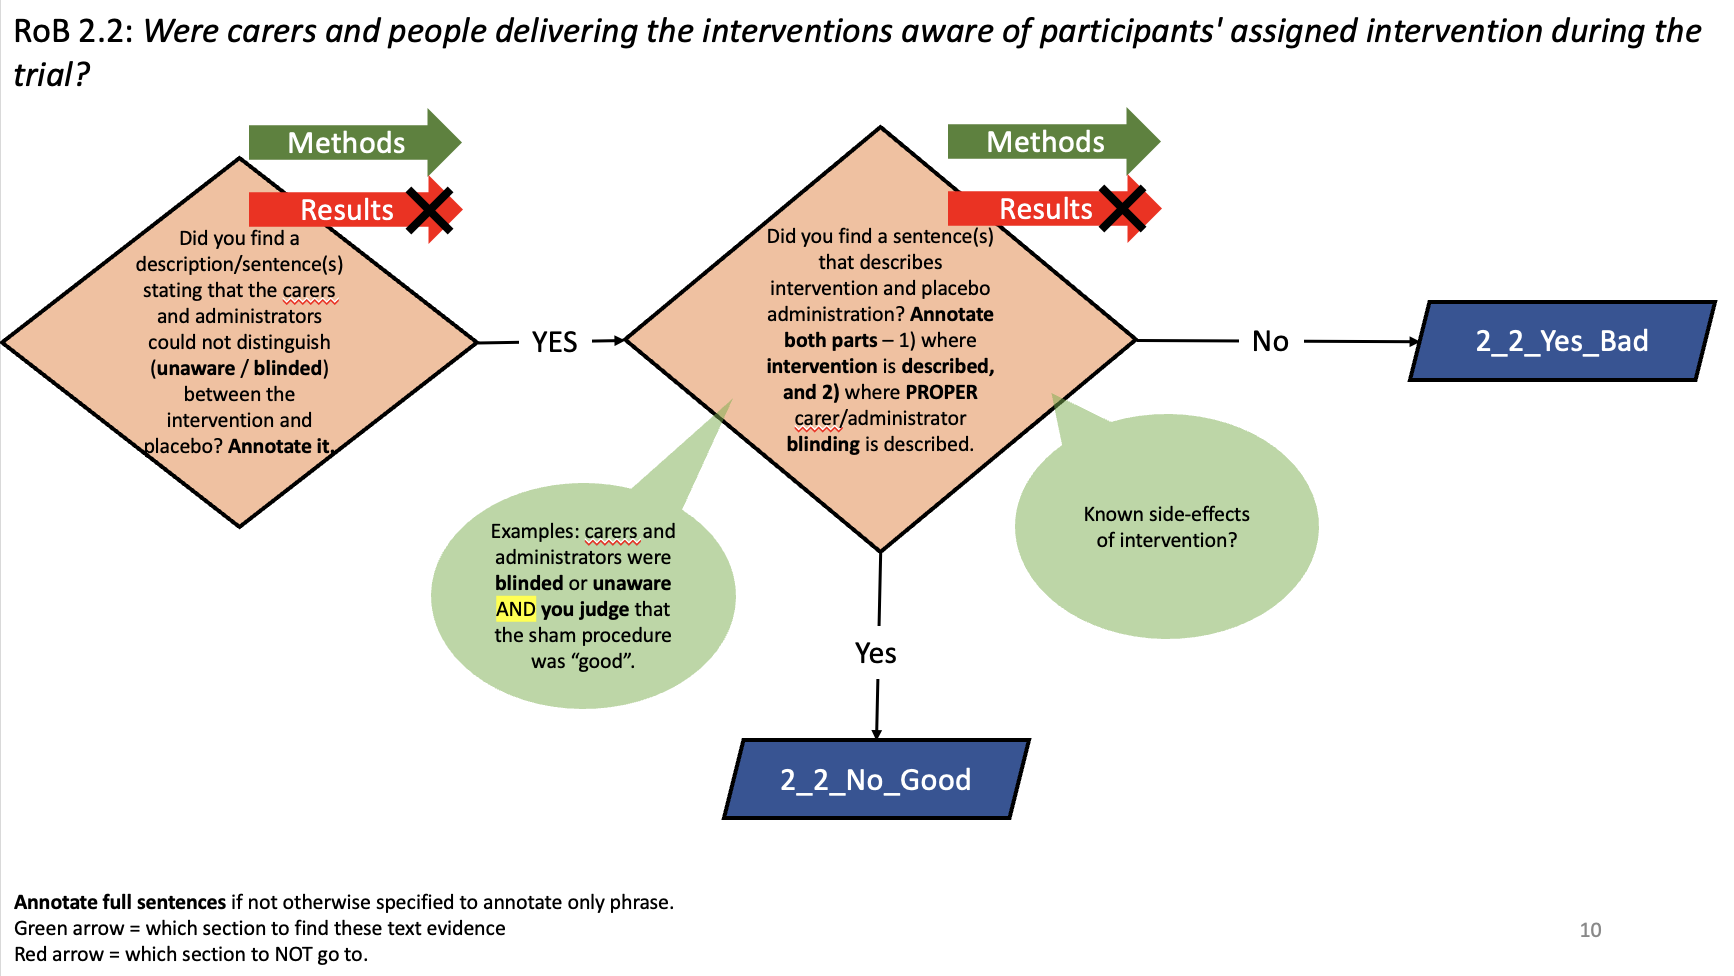
\includegraphics[width=\textwidth]{figures/2_2.png}
    \caption{Annotation instructions for the RoB 2.2 signalling question.}
    \label{fig:2_2}
\end{figure}
%


%
%
%
\subsection*{Signalling question - 2.3}
\label{subsec:2_3}
%
Follow the Flowchart~\ref{fig:2_3} for annotation instructions of the signalling question, ``Were there deviations from the intended intervention that arose because of the trial context?''.
%
\begin{figure}[hbt]
    \centering
    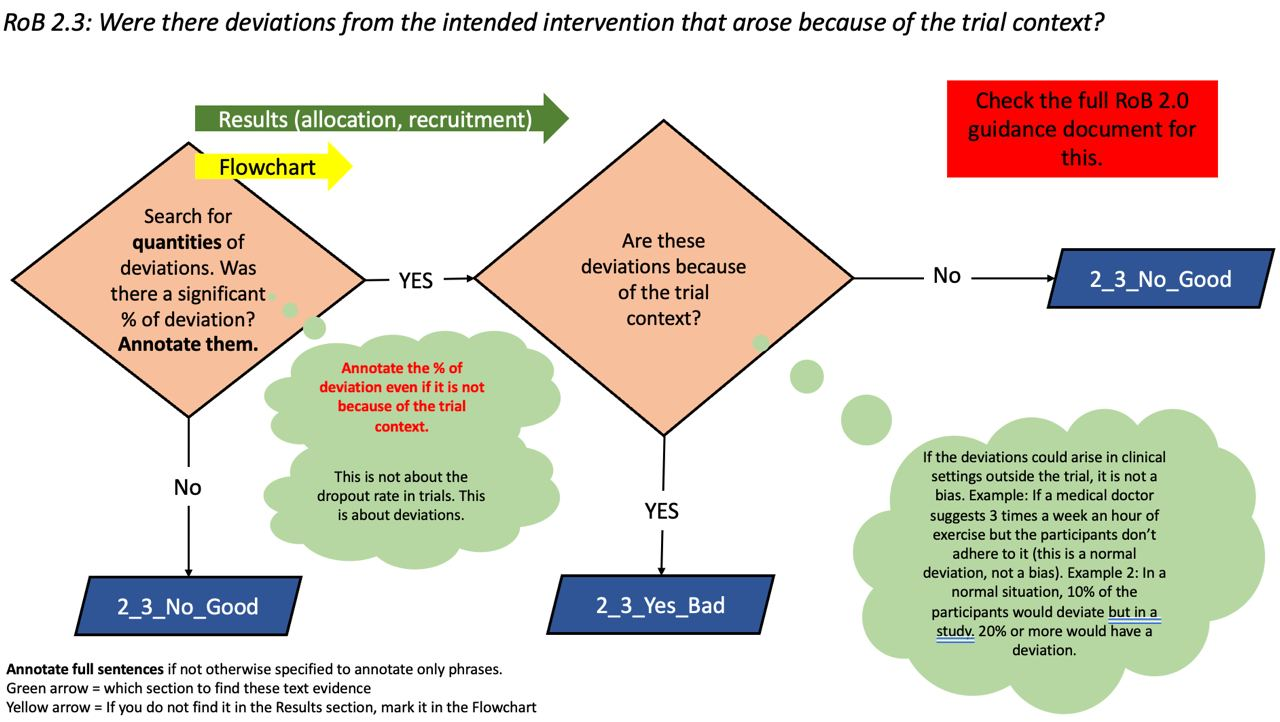
\includegraphics[width=\textwidth]{figures/2_3.jpg}
    \caption{Annotation instructions for the RoB 2.3 signalling question.}
    \label{fig:2_3}
\end{figure}
%


The first diamond in the flowchart asks the annotators to search for quantities of deviation with a thought bubble hinting to them that these deviations are not the dropout rate in the trial.
The diamond element also hints to the annotators that they can find this information in the text of the Results section, either within the allocation paragraph or the recruitment paragraph (green-coded arrow).
If the information was not found within the Results section, look for it in the flowchart (either the flowcharts themselves or their captions).
If no percentage deviation or the absolute number of deviations were identified in the text, do not annotate anything, and this document will be automatically marked as a ``no information'' for this signalling question following the arrow of ``no''.
If the percentage of deviation was identified, then annotate the full sentence where this information is found.
Next, go to the next diamond following the ``yes'' flow and judge whether these deviations were due to the trial context.
If these deviations arose due to trial context, mark the annotated sentence(s) as ``2.3 Yes Bad'' and ``2.3 No Good'' otherwise.
Additionally, if you identify the reason for your choice of ``no good'' and ''yes bad'' mark the sentences denoting the reason for your choice.
In conclusion, you need to make a second annotation in this case if you have sentences to support your reason.
Now the second diamond is quite subjective and you might not find the information, but at least you will have the annotated information about the percentage/number of deviations which could be used to train the machine learning models.
We let the reviewers be a judge of the trial context once they discover the deviation information.
Ultimately, the review of deviations and trial context is subjective, but the annotated information can be used to train machine learning models.
%
%
%
\subsection*{Signalling question - 2.4 }
%
For annotation instructions for this signalling question, ``Were these deviations likely to have affected the outcome?'' follow the Flowchart~\ref{fig:2_4}.
%
\begin{figure}[hbt]
    \centering
    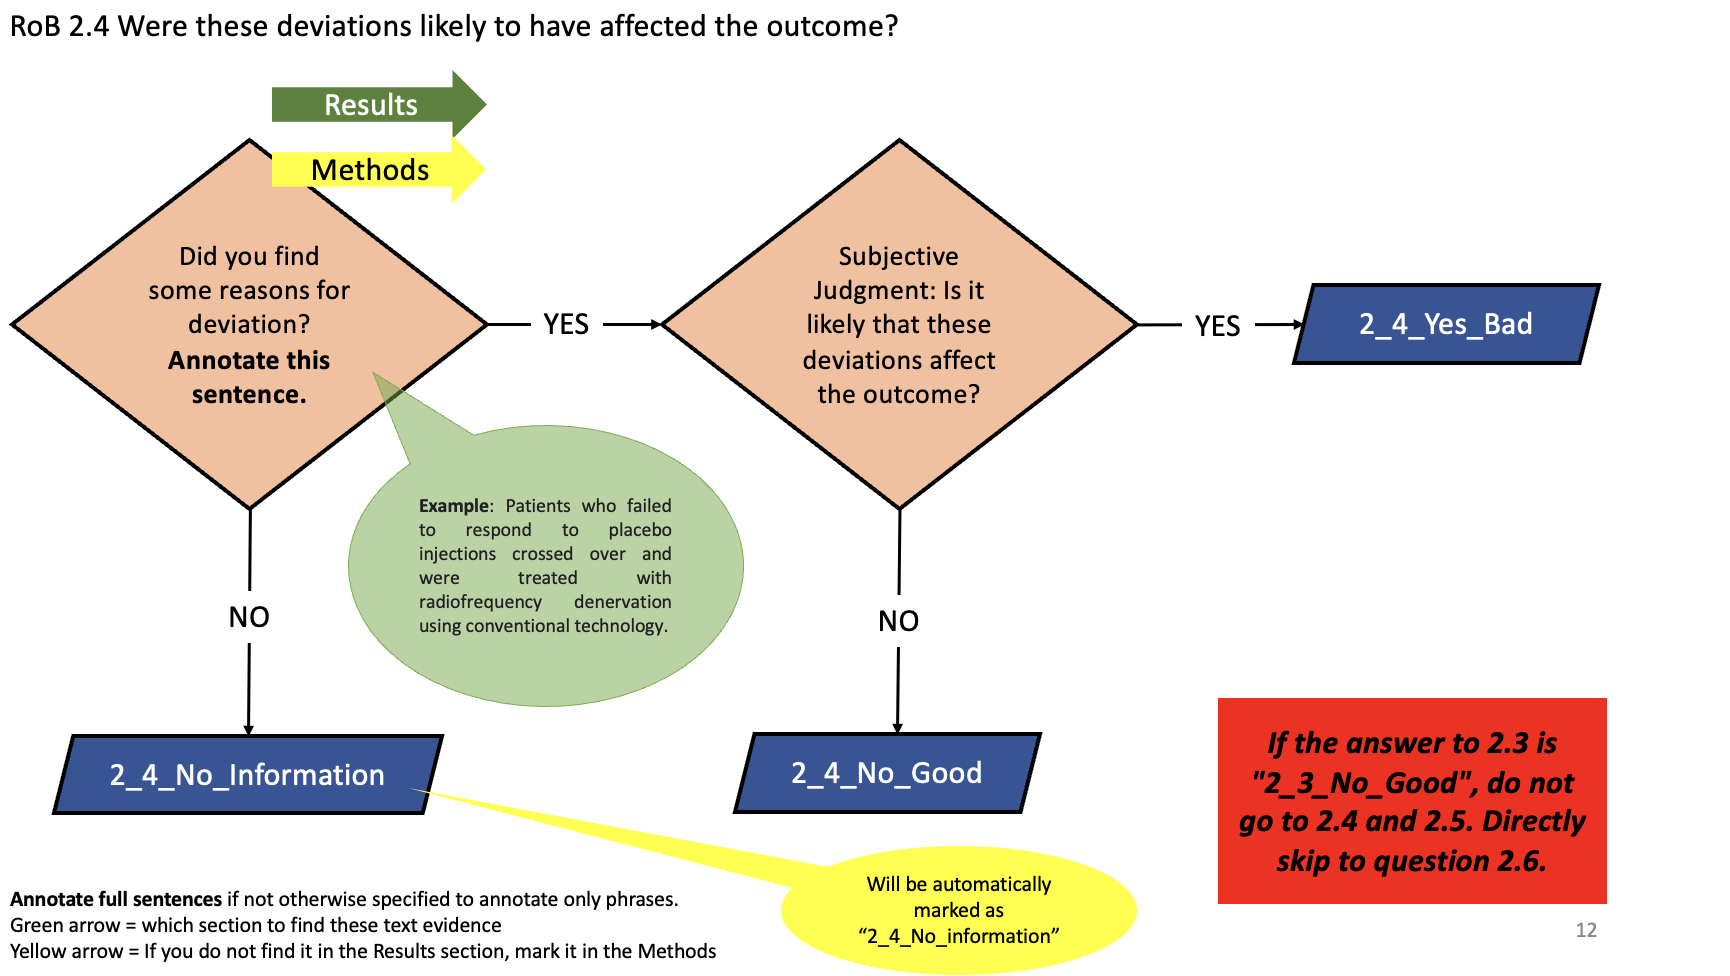
\includegraphics[width=\textwidth]{figures/2_4.png}
    \caption{Annotation instructions for the RoB 2.4 signalling question.}
    \label{fig:2_4}
\end{figure}
%
Do not annotate for this question if the answer to the previous question was ``2.3 No Good''; otherwise, follow the instructions below.
In randomized clinical trials, deviations from the planned study protocol may occur for various reasons, such as the participant not following the intervention as intended or the trial site not adhering to the study procedures.
These deviations are known as "protocol deviations" or "protocol violations."
The question "Were these deviations likely to have affected the outcome?" in the revised Cochrane RoB 2.0 tool refers to whether the protocol deviations had the potential to influence the study results.
The aim of this question is to assess the RoB due to the protocol deviations, which may have introduced systematic error or affected the internal validity of the study.
If the deviations were unlikely to have affected the study outcome, then this question would be answered with "No."
However, if the deviations were likely to have affected the study outcome, then this question would be answered with "Yes," indicating that the study is at high risk of bias.
If it is unclear whether the deviations affected the outcome, the answer would be "Some concerns."
To annotate the information from the previous question, we identify the percentage of deviation (a number) and annotate it, while for this question, we look for the reasons for these deviations and annotate them.
The reasons could be found in either the Results section or in the Method section if not in the Results section.
If you identify the reason for this deviation and mark it, then follow the path along ``yes'' and judge whether these deviations could affect the outcome.
If they do, mark the annotated reason for deviation as ``2.4 Yes Bad'' and ``2.4 No Good''otherwise.
For example, this sentence from Osteras 2019 Patient Reporting Quality of Care 6months IAA Hilfiker Sattelmayer with Protocol.pdf ... "['Two patients in the control group receiving physiotherapy (usual care) erroneously attended the PT-led education and exercise programme after their PT had attended the workshop.']" says that some participants went to different therapy "by error/mistake" which is a reason for the deviation, but as it was a small deviation, the annotator marked it as "no good".
%
%
%
\subsection*{Signalling question - 2.5 }
%
For annotation instructions for this signalling question, ``Were these deviations from the intended intervention balanced between groups??'' follow the Flowchart~\ref{fig:2_5}.
%
\begin{figure}[hbt]
    \centering
    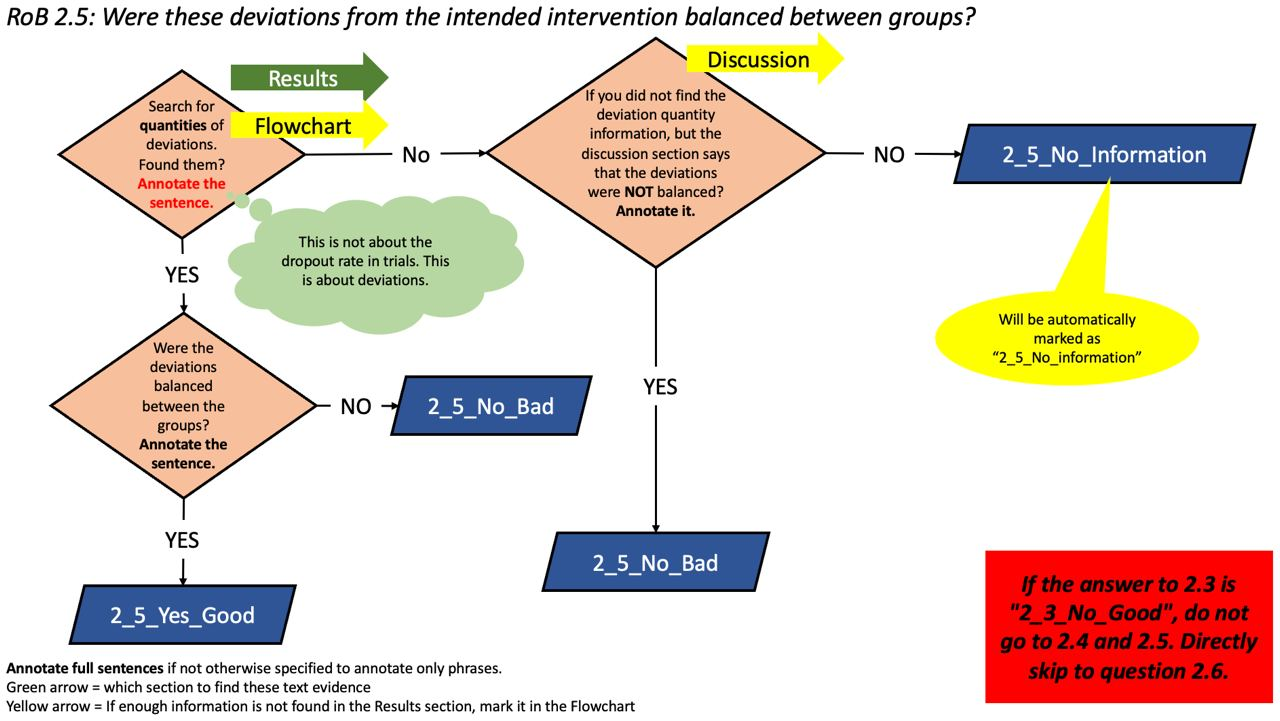
\includegraphics[width=\textwidth]{figures/2_5.jpg}
    \caption{Annotation instructions for the RoB 2.5 signalling question.}
    \label{fig:2_5}
\end{figure}
%
In the context of a randomized controlled trial (RCT), the intended intervention refers to the intervention that was supposed to be given to the study participants according to the study protocol. However, sometimes deviations from the intended intervention may occur due to various reasons, such as participant non-compliance or study staff error.

The question "Were these deviations from the intended intervention balanced between groups?" is asking whether any deviations from the intended intervention were similar in frequency and severity across the different study groups (i.e., intervention group and control group) or whether one group had a greater number or severity of deviations than the other.

Balanced deviations between groups are important for maintaining the internal validity of the study. If one group had a higher number or severity of deviations from the intended intervention than the other, it could potentially introduce bias and confound the results of the study. Therefore, it is important to assess whether deviations from the intended intervention were balanced between the groups when evaluating the risk of bias in an RCT.

The first diamond in the flowchart asks the annotators to search for quantities of deviation with a thought bubble hinting to them that these deviations are not the dropout rate in the trial (to understand the difference between deviations and dropout, refer to subsection~\ref{subsec:2_3}).
The main hook point is to identify quantities or numbers that show some kind of deviation from the intended intervention.
If the deviations were balanced between the groups, mark the annotated deviations as ``2.5 Yes Good'' and ``2.5 No Bad'' otherwise.
Now if you did not find any quantification of the deviations but found the text in the Discussion section saying that the deviations were not balanced, then mark such text in the discussion as ``2.5 No Bad''.
If no text is marked, the document for this signalling question will be marked with a no information label.
%
%
%
%
\subsection*{Signalling question - 2.7 }
%
For annotation instructions for this signalling question, ``Was there potential for a substantial impact (on the result) of the failure to analyse participants in the group to which they were randomized?'' follow the Flowchart~\ref{fig:2_7}.
%
\begin{figure}[hbt]
    \centering
    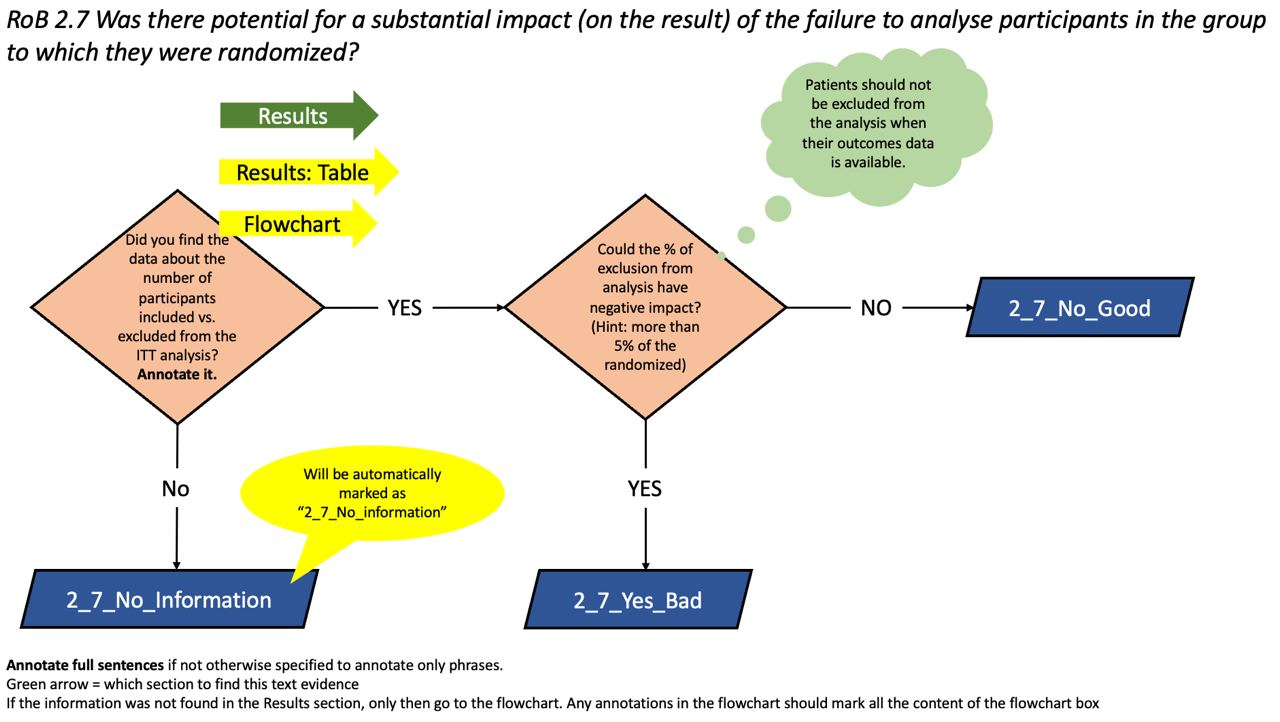
\includegraphics[width=\textwidth]{figures/2_7.jpg}
    \caption{Annotation instructions for the RoB 2.7 signalling question.}
    \label{fig:2_7}
\end{figure}


The question ``Was there potential for a substantial impact (on the result) of the failure to analyze participants in the group to which they were randomized?'' in the Cochrane Risk of Bias (RoB) 2.0 tool refers to the risk of bias associated with deviations from the intended analysis plan in a randomized controlled trial (RCT).

In an RCT, participants are usually randomized to receive either the intervention being tested or a control intervention. The analysis plan is typically based on the assumption that all participants will be analyzed according to the group to which they were randomized. However, there may be instances where participants are not analyzed in the group to which they were randomized, for example, if they dropped out of the study or if they switched groups. This is known as a deviation from the intended analysis plan.

The question is asking whether this deviation from the intended analysis plan could have had a substantial impact on the study results. If there is a potential for a substantial impact, then there is a high risk of bias. For example, if a large proportion of participants in the intervention group dropped out of the study, but all participants in the control group were analyzed, this could lead to an overestimation of the treatment effect. Similarly, if participants switched groups, this could lead to an underestimation or overestimation of the treatment effect.

Therefore, this question is important for assessing the risk of bias associated with deviations from the intended analysis plan in an RCT, and it helps to ensure that the study results are reliable and valid.


The analysis we focus on this question is ITT or intent-to-treat analysis.
The first diamond asks the annotators to find the number of people included in the ITT analysis vs. the number of people randomized to each of the intervention/comparator groups. 
If this information (number of people included in the analysis vs number of people randomized to each group) is found, annotate it and follow the ``yes'' flow in the diagram.
Now examine whether the percentage of participants excluded from the ITT analysis could have had a negative impact.
We also include a hint here, and if more than 5\% of randomized participants were excluded from ITT analysis, we ask the annotators to mark the text as ``2.7 Yes Bad'' and ``2.7 No Good'' otherwise.

A good agreement is only if we mark captions in flowcharts.
The first preference to find this information is the results section, and if found, then mark the full sentence in the text.
If the information is not found in the results section, mark the text in the table.
If the information is to be found nowhere except in a flowchart, mark the caption of the flowchart.
However, ensure that the flowchart annotation is your last resort.

If you find it in the flowchart, mark the caption and also ``included n=XX for ITT''. % Unfortunately, you cannot mark the flowchart because the new tool does not allow image annotation

Sometimes there could be disagreements here. Let's take for example, Solomons\_2020\_VISA\_A\_12months\_IAA\_Hilfiker\_Sattelmayer\_with\_Protocol.pdf where Martin marks "We did not impute or replace any missing values but rather fitted all the available data to the model" as No good. 
However, what does the phrase "all the available data" mean? Maybe only 70\% of the outcomes data was available.
%
%
%
\subsection*{Signalling question - 3.2 }
%
For annotation instructions for this signalling question, ``Is there evidence that the result was not biased by missing outcome data?'' follow the Flowchart~\ref{fig:3_2}.
%
\begin{figure}[hbt]
    \centering
    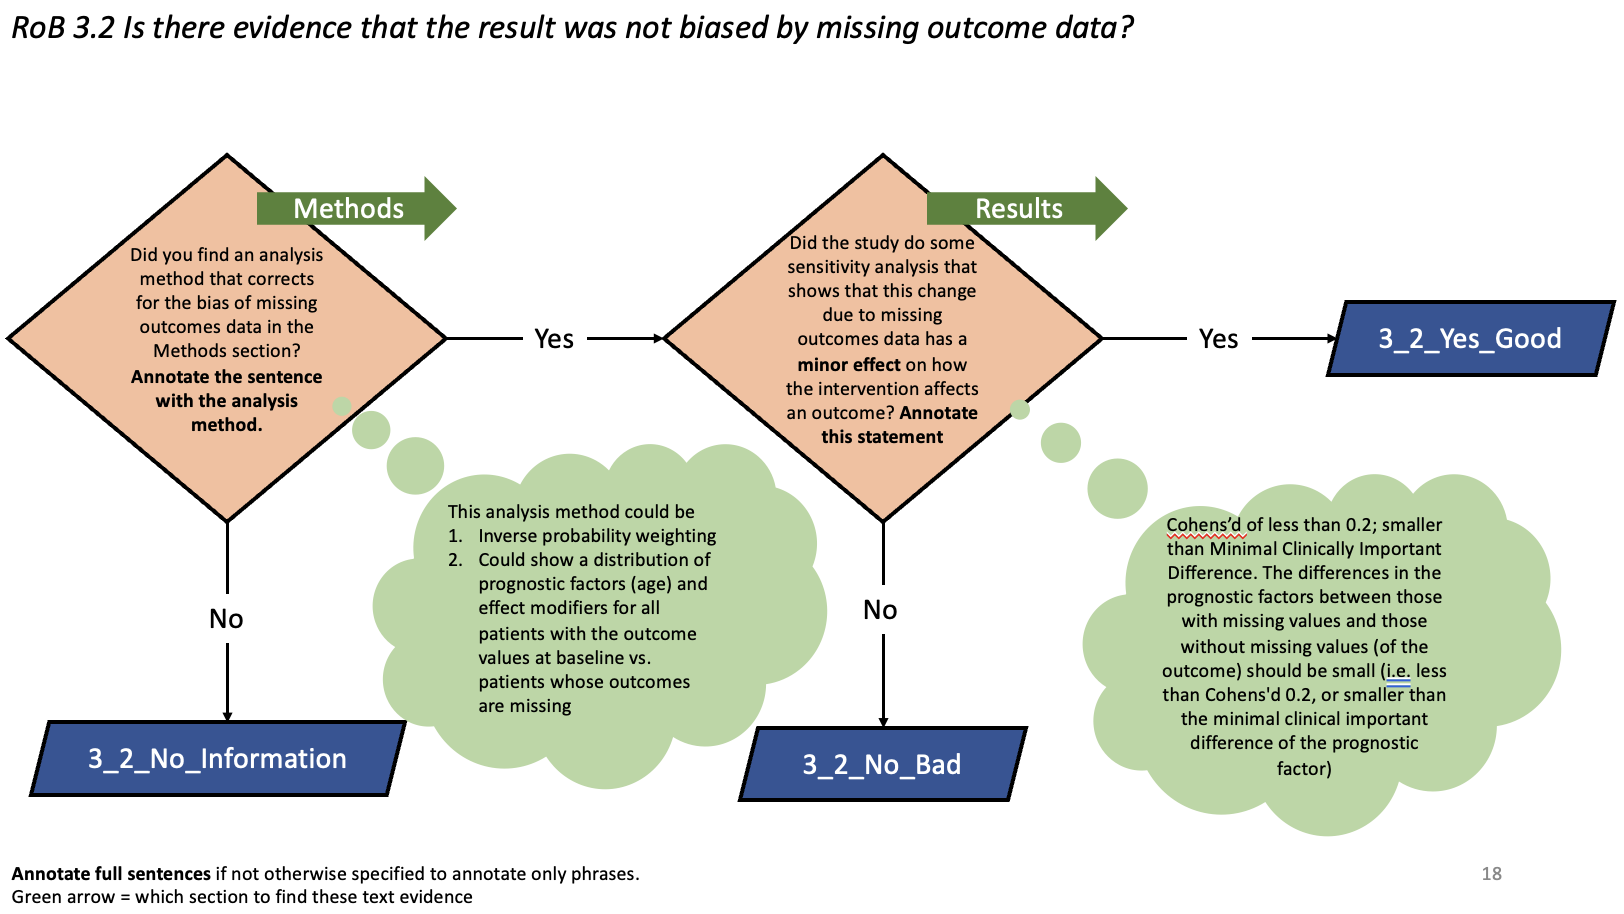
\includegraphics[width=\textwidth]{figures/3_2.png}
    \caption{Annotation instructions for the RoB 3.2 signalling question.}
    \label{fig:3_2}
\end{figure}
%
When answering this question, researchers evaluate whether the missing outcome data could have influenced the study's results in a biased manner.
Missing outcome data can occur when participants drop out of a study, fail to provide data for certain outcomes, or when data is not collected as planned.
The concern is that the missing data may introduce bias if it is related to the treatment being studied or if it differs systematically between the treatment groups.
To determine if there is evidence that the result was not biased by missing outcome data, researchers typically assess the amount of missing data and whether it is evenly distributed across different study groups.
If there is a significant amount of missing data, especially if it is related to the outcomes being measured, it may increase the risk of bias.
Researchers evaluate the strategies employed to handle missing data.
This may involve techniques such as imputation (replacing missing values with estimated values) or sensitivity analyses to assess the impact of missing data on the results.
To annotate for this signalling question, the annotators should specifically look for the anaylsis method that was used to handle or correct for the missing outcomes data.
This analysis method could be, for example, Multiple Imputation (MI), Inverse Probability Weighting (IPW), Weighted Estimating Equations (WEE), Pattern Mixture Models (PMM).
The first diamond asks the annotators to look for this method.
If the name of the analysis method is found, go to the next diamond which instructs the annotator to identify any method that was used to conduct sensitivity analysis.
Did the study do some sensitivity analysis that shows that this change due to missing outcomes data or the different analysis methods used have a minor effect on how the intervention affects an outcome?
Then annotate these sentences containing the analysis method and sensitivity analysis and mark them with ``3.2 Yes Good''.
By conducting sensitivity analyses, researchers can gain insight into the potential impact of missing data on the study's findings. This information helps to address concerns regarding bias and strengthens the overall validity and reliability of the study results.
If no sensitivity analysis was done then mark the sentence containing method used to handle the missing data and label it as ``3.2 No Bad''.
%
%
%
\subsection*{Signalling question - 3.3 }
%
RoB 3.3 focuses on whether the missing data is related to the true value of the outcome. For example, if participants with higher or lower values of the outcome are more likely to drop out or have missing data, this could introduce bias. In this case, the missing data could depend on the true value of the outcome, and the results of the study could be biased.

To answer this question, reviewers need to assess whether there is a potential relationship between the missing data and the true value of the outcome. This can be done by examining the reasons for missing data and analyzing whether the missing data is related to other participant characteristics or study factors.

If the answer to RoB 3.3 is judged as "low risk of bias," it means that there is little risk that the missing data could have biased the study findings. If the answer is "high risk of bias," it means that there is a significant risk of bias due to missing outcome data, and the study results should be interpreted with caution.
%
%
%
%%===========================================================================================%%
%% If you are submitting to one of the Nature Portfolio journals using the eJP submission   %%
%% system, please include the references within the manuscript file itself. You may do this  %%
%% by copying the reference list from your .bbl file, paste it into the main manuscript .tex %%
%% file, and delete the associated \verb+\bibliography+ commands.                            %%
%%===========================================================================================%%

\bibliography{sn-bibliography.bib}% common bib file
%% if required, the content of the .bbl file can be included here once bbl is generated
%%\input sn-article.bbl


\end{document}
